\documentclass[11pt]{article}

\usepackage{parskip}
\usepackage{graphicx}
\usepackage{amsmath}
\usepackage{listings}

\usepackage[T1]{fontenc}
\usepackage{lmodern}
\usepackage[autostyle, english = american]{csquotes}
\MakeOuterQuote{"}

\usepackage{pythonhighlight}

% Margins
\topmargin=-0.45in
\evensidemargin=0in
\oddsidemargin=0in
\textwidth=6.5in
\textheight=9.0in
\headsep=0.25in

\title{605.744: Information Retrieval \\ Programming Assignment \#2: Inverted Files}
\author{Sabbir Ahmed}
\date{\today}

\begin{document}
\maketitle	

\section{Introduction}
This paper describes the enhancements and features added to the Information Retrieval program started in Assignment 1. Modifications include improvement in performance and efficiency in normalizing text and generating statistics from the pre-generated corpus and addition of binary inverted files.

\section{Technical Background}
All of the source code is in Python 3.10. The program is split into several modules and follows an object oriented structure. The following is the directory structure of the source code:

% .
% ├── bin
% │   ├── headlines_dict.json
% │   └── headlines_if.bin
% ├── ir
% │   ├── files.py
% │   ├── __init__.py
% │   ├── invertedfile.py
% │   ├── lexer.py
% │   ├── normalize.py
% │   └── packer
% ├── run.py
% ├── stats
% │   ├── headlines_df.json
% │   ├── headlines_stats.txt
% │   └── headlines_tf.json
% ├── test.py
% └── tmp
%     └── headlines_tdt.txt


\begin{figure}[!ht]
    \centering
    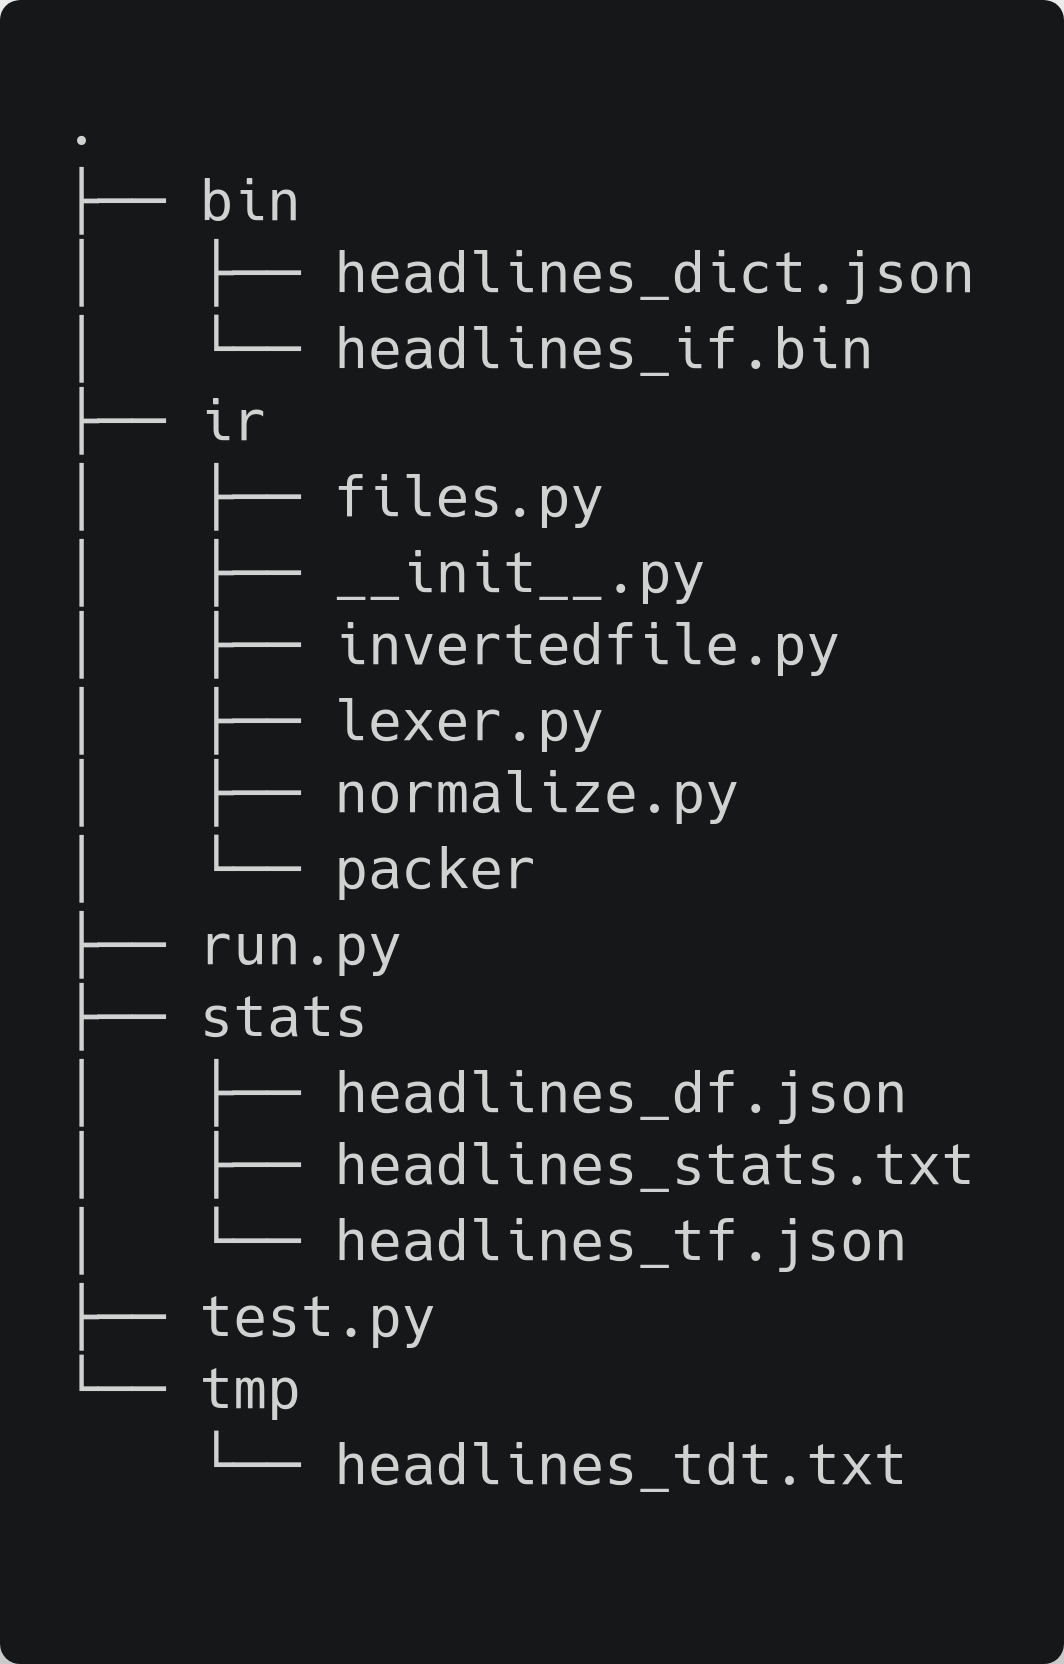
\includegraphics[scale=0.2]{statics/dirtree.png}
    \caption{Directory Hierarchy of Assignment 2}
\end{figure}

The source code for all of the files are attached in Appendix \ref{appendix:src}.

The total number of non-empty lines of code for the program doubled to just under 400. However, the average execution time to process the sample files reduced to 37 seconds. 

\begin{figure}[!ht]
    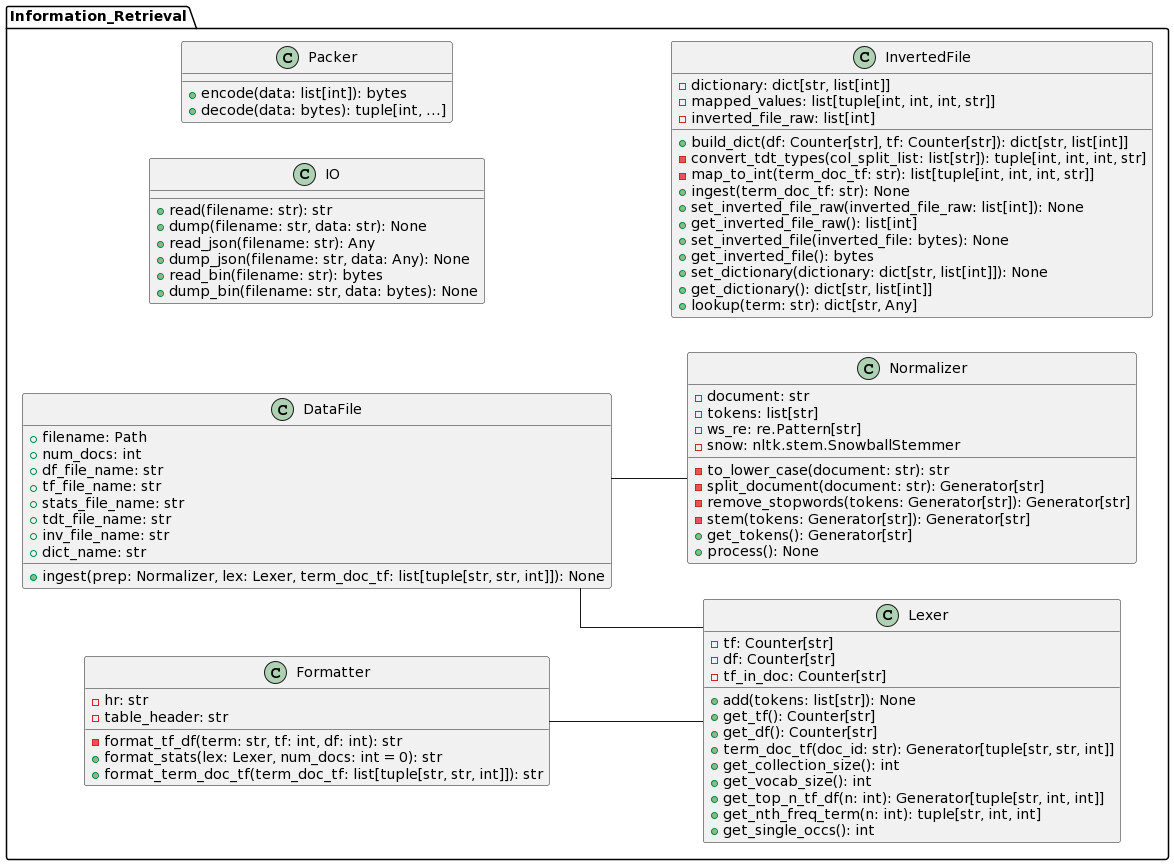
\includegraphics[scale=0.43]{statics/uml.png}
    \centering
    \caption{UML of Information Retrieval}
\end{figure}

\subsection{Existing Classes}

\subsubsection{Driver} \label{sec:driver}
The driver script for the program is split between \texttt{run.py} and \texttt{test.py}. The former script, while maintaining the responsibility for the same list of tasks as the previous iteration, also generates the binary inverted files and dictionaries for the sample corpus and saves it to disk. The latter script loads the inverted files and dictionaries and looks up the test terms as specified in the prompt.

\subsubsection{\texttt{normalize.Normalizer}}
The \texttt{Normalizer} class received the following modifications:

\begin{enumerate}
    \item expansion of word contractions was replaced by removing all of the stopwords. The stopwords are a mixture of tokens from \texttt{nltk.corpus.stopwords.words("english")} and the contractions hash table keys. The larger list of "STOPWORDS" is represented as a Python set() object for efficient lookups.

    \item all of the normalizing methods accept generators as input to improve performance on memory.
\end{enumerate}

\subsubsection{\texttt{lexer.Lexer}}
The \texttt{Lexer} class received the following modifications:
\begin{enumerate}
    \item the Counter object \texttt{tf\_in\_doc} was added to maintain a term-frequency of the current document. This addition allows for the new method \texttt{term\_doc\_tf(doc\_id: str)} that generates tuples of \texttt{(term-string, doc-ID, term-document-frequency)}. These tuples are saved on disk in files named "sample\_tdt.txt" for further sorting and processing to generate the inverted files.
\end{enumerate}

\subsection{\texttt{New Classes}}

\subsubsection{\texttt{invertedfile.InvertedFile}}
The \texttt{InvertedFile} class is responsible for building the binary inverted files and dictionaries. The class ingests the "sample\_tdt.txt" files, sorts (in memory) the tuples as detailed in the prompt, and converts the values into 4-byte integer formats. The class also provides a method to look up tokens in the generated inverted files and dictionaries.

\subsubsection{\texttt{packer.Packer}}
The \texttt{Packer} class is responsible for encoding and decoding fixed-format binary data.

\subsubsection{\texttt{files} Classes}
The \texttt{IO} class was decoupled from \texttt{Lexer} and \texttt{Normalizer} and further split into 2 additional classes, \texttt{Formatter} and \texttt{DataFile}. These classes provide support for file utility functions in the program, including reading and writing to plain files, JSON files, and binary files, formatting statistics outputs, generating file paths, etc.

\section{Statistics and Observations}
With the modifications made to the text normalization process, the statistics generated from the input file have changed. The new top 10 more frequent tokens now include "market", "announc", and "report", which are terms that expected in headlines.

In terms of the inverted files and dictionaries, the space they occupy on disk combined are significantly lower than the original document.

\begin{table}[h]
    \begin{center}
        
        \begin{tabular}{| l | r | l |}
        \hline
        \textbf{File} & \textbf{Size (in bytes)} & \textbf{Description} \\
        \hline
        headlines.txt & 39381610 & Input corpus file \\
        headlines\_dict.json & 4275427 & Generated dictionary JSON file \\
        headlines\_if.bin & 27774312 & Inverted binary file \\
        \hline
        \end{tabular}

    \end{center}
    \caption{Sizes of Files Computed Through the \texttt{stat} Command on a Debian Based Linux}

\end{table}

\section{Testing}
The tests described by the prompt were performed via the \texttt{test.py} driver script. The tokens to look up had to first be normalized through the \texttt{Normalizer} class.

\begin{lstlisting}[style=mypython,
    caption=Test 1: Document frequency and postings list for the terms: "Heidelberg"\, "cesium"\, "Trondheim"\, "crustacean"]
# NOTE: the normalization stems "crustacean" to "crustacea"
# and "crustaceans" to "crustacean"
tokens1 = normalize_test_terms(
    prep, ("Heidelberg", "cesium", "Trondheim", "crustaceans")
)
results1 = read_inverted_file(
    invf,
    tokens1,
    ("term", "postings", "postings_len"),
)
\end{lstlisting}

\begin{figure}[!ht]
    \centering
    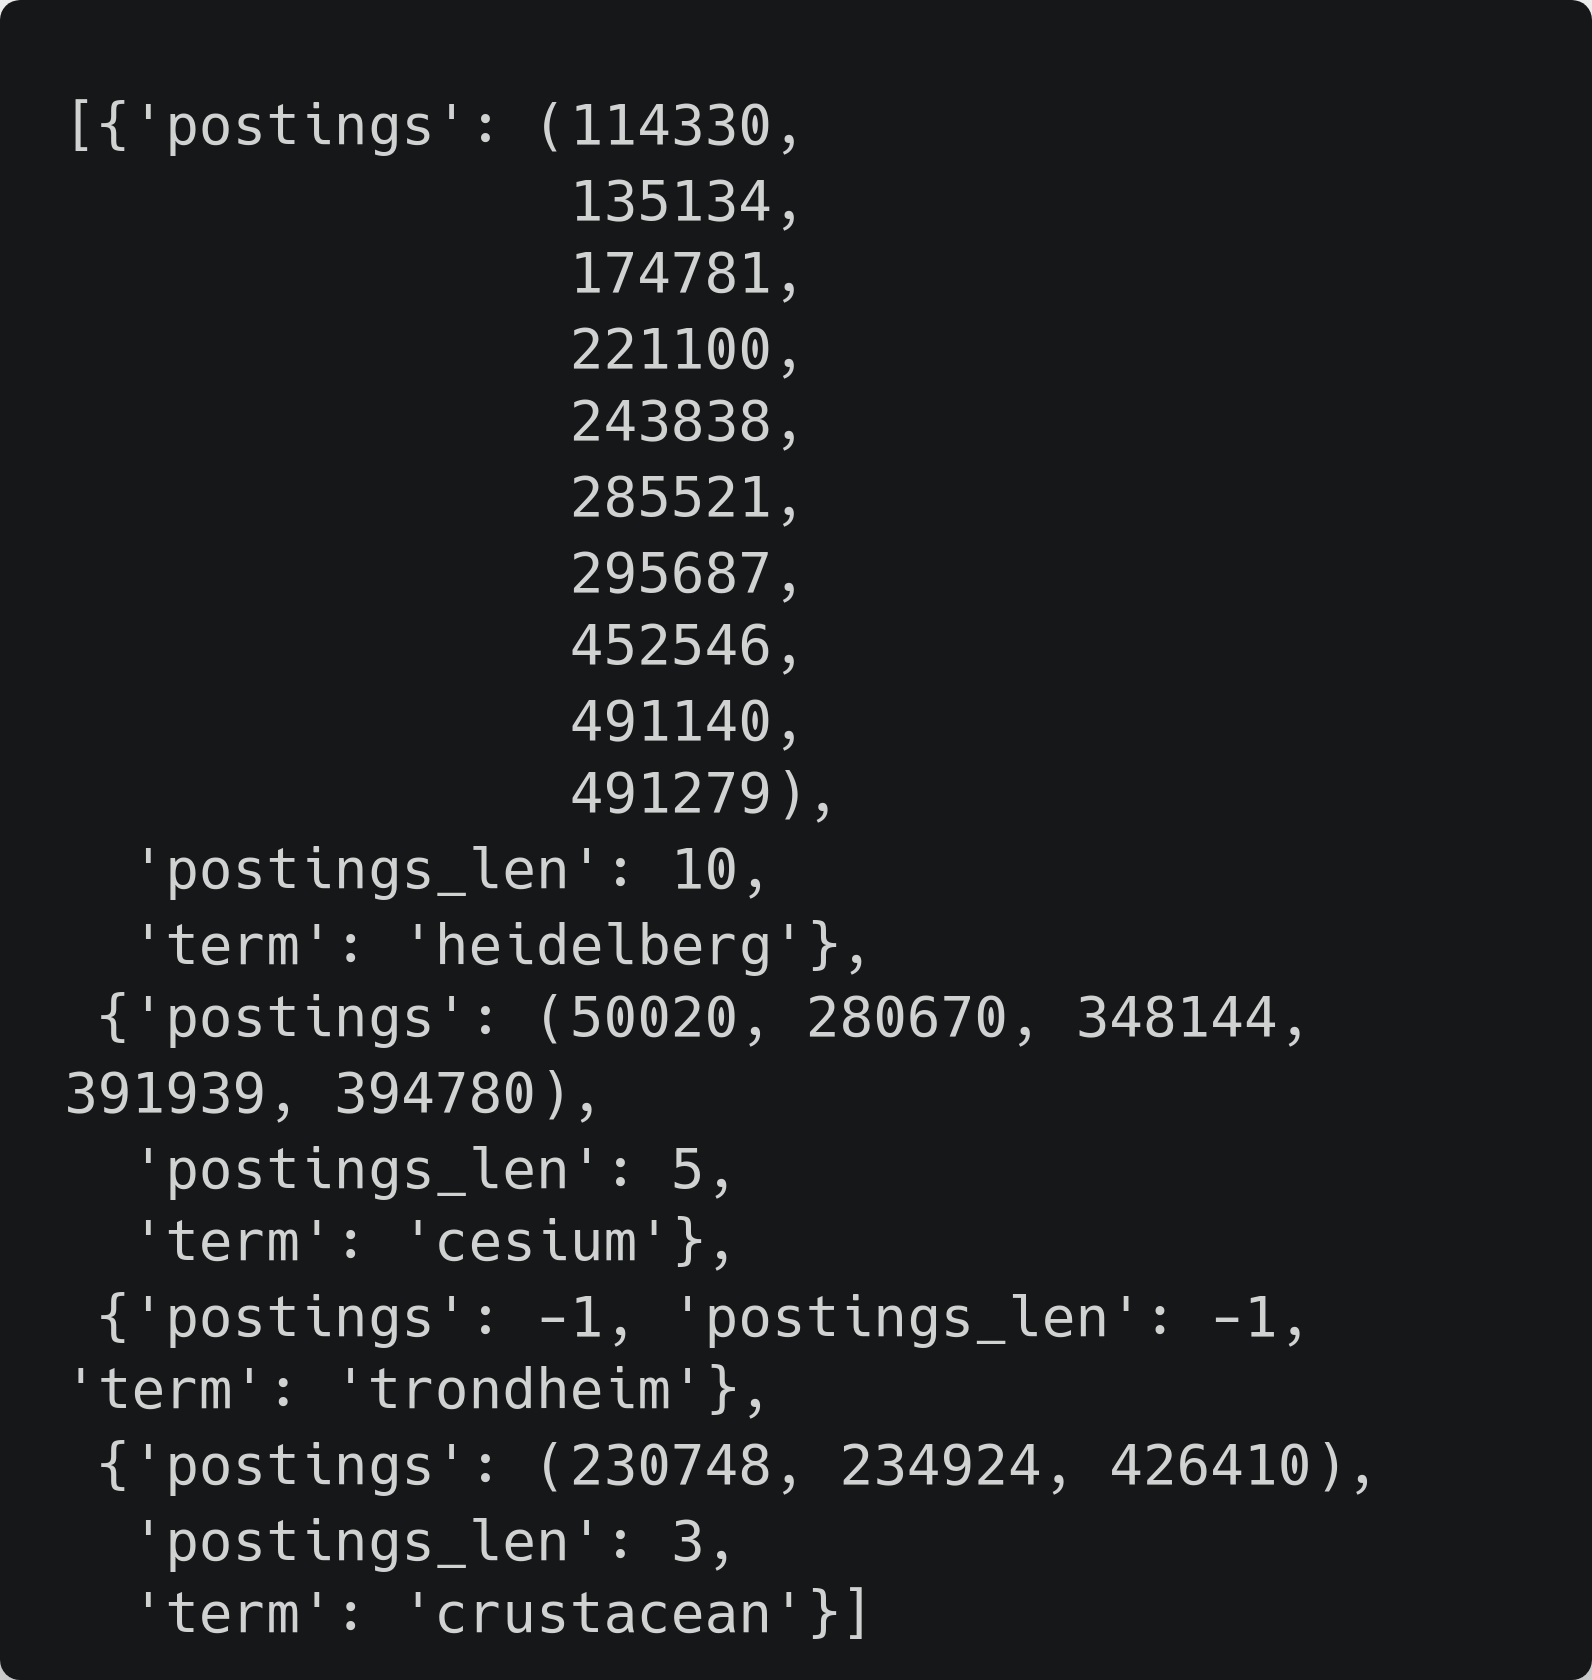
\includegraphics[scale=0.15]{statics/test1.png}
    \caption{Output of Test 1}
\end{figure}
\clearpage
\newpage

\begin{lstlisting}[style=mypython,caption=Test 2: Document frequency for the words: "Hopkins"\, "Stanford"\, "Brown"\, and "college"]
tokens2 = normalize_test_terms(
    prep, ("Hopkins", "Stanford", "Brown", "college")
)
results2 = read_inverted_file(invf, tokens2, ("term", "postings_len"))
\end{lstlisting}
% \clearpage
% \newpage

\begin{figure}[!ht]
    \centering
    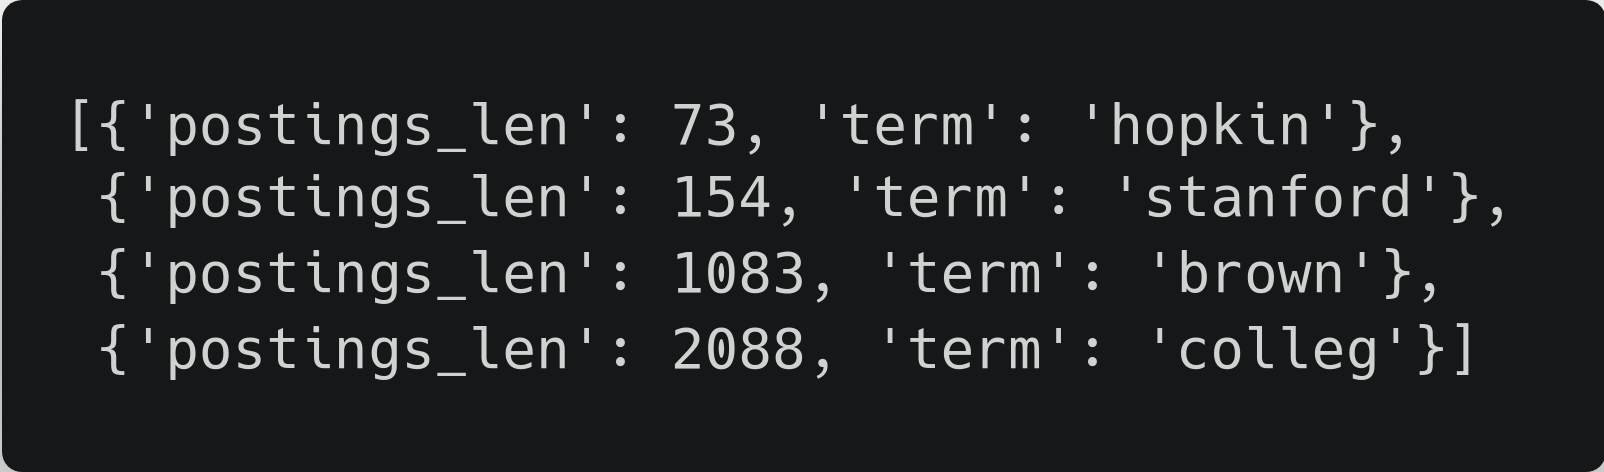
\includegraphics[scale=0.15]{statics/test2.png}
    \caption{Output of Test 2}
\end{figure}

\begin{lstlisting}[style=mypython,caption=Test 3: docids for documents that have both "Elon" and "Musk"]
# NOTE: the normalization stems "Musks" to "Musk"
tokens3 = normalize_test_terms(prep, ("Elon", "Musks"))
results3 = read_inverted_file(invf, tokens3, ("postings",))
elon, musk = results3
elon_postings, musk_postings = set(elon["postings"]), set(musk["postings"])
elon_musk_postings = elon_postings & musk_postings
\end{lstlisting}

\begin{figure}[!ht]
    \centering
    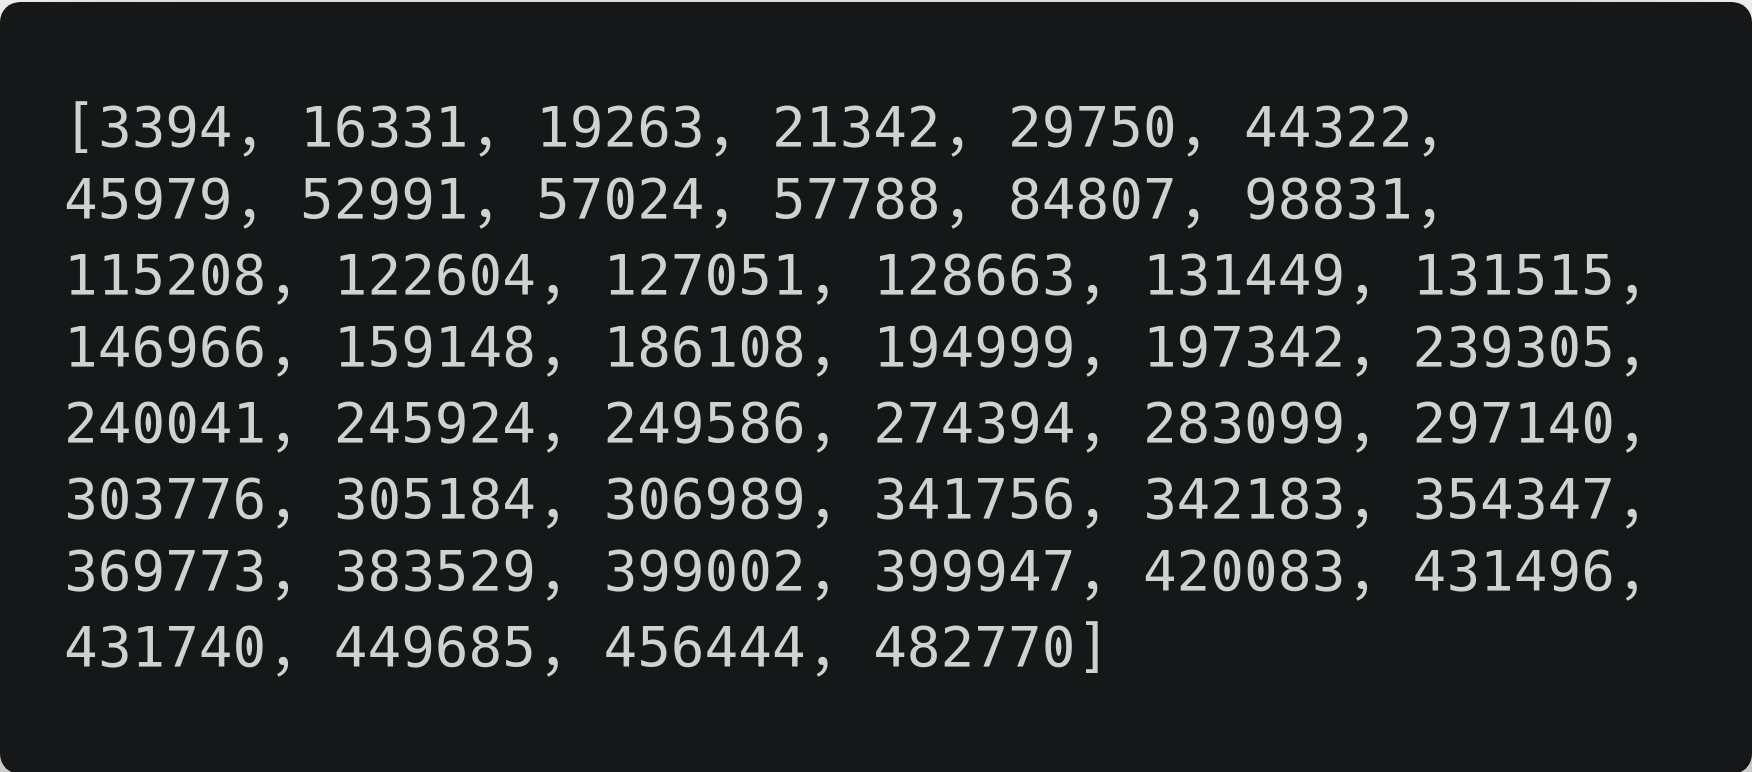
\includegraphics[scale=0.15]{statics/test3.png}
    \caption{Output of Test 3}
\end{figure}

\appendix

\section{Source Code} \label{appendix:src}

\inputpython{./ir/files.py}{./ir/files.py}
\inputpython{./ir/invertedfile.py}{./ir/invertedfile.py}
\inputpython{./ir/normalize.py}{./ir/normalize.py}
\inputpython{./ir/lexer.py}{./ir/lexer.py}
\inputpython{./ir/packer.py}{./ir/packer.py}

\inputpython{./run.py}{./run.py}
\inputpython{./test.py}{./test.py}

\section{Outputs} \label{appendix:outputs}

\lstinputlisting[caption=Statistics of 'headlines.txt',basicstyle=\small]{./stats/headlines_stats.txt}

\end{document}
